%% pdflatex
%% Slides for EEE5112 Course 2012
%% M.R. Inggs   started 28/04/2012
%% S.L. Coetzee removed some errors 22/09/2015
%% Course notes V0.0

%% IEEE Radar Conf Paper
%% 9 April 2019

\def\lecNo{\copyright~UCT~IEEE~RadarConf2019}  % Which lecture
\def\version{V0.1}
%% Put the code for your course here: CourseCode-Year-Version
%% 

\documentclass[xcolor=dvipsnames]{beamer}
\let\Tiny=\tiny
% Bring in all the style sheets
%% Common material for slides.
%% Version 0.0 by MRI 8/05/12
%% Version 0.1 updated by MRI to sort out \subcaption.


%\documentclass[xcolor=dvipsnames]{beamer}
\usepackage{xcolor}

%\usepackage{caption}
\usepackage{subcaption}
\captionsetup{compatibility=false}

% Special colours
\setbeamercolor{uppercol}{fg=black,bg=blue!40}
\setbeamercolor{lowercol}{fg=black,bg=blue!10}


% Setup appearance:

\usetheme{Singapore}
\usefonttheme[onlylarge]{structurebold}
\setbeamerfont*{frametitle}{size=\normalsize,series=\bfseries}
\setbeamertemplate{navigation symbols}{}


\pgfdeclareimage[height=1.2cm]{university-logo}{figs/UCT_logocircless_t}
\logo{\pgfuseimage{university-logo}}



\setbeamertemplate{footline}[text line]{
\parbox{\linewidth}{\vspace*{-8pt}\lecNo\version\hfill\insertpagenumber~of~\pageref{lastpg}}}
%\parbox{\linewidth}{\vspace*{-8pt}\version\hfill\insertshortauthor\hfill\insertpagenumber~of~\pageref{lastpg}}}
\setbeamertemplate{navigation symbols}{}

\setbeamertemplate{bibliography item}[text]  % to obtain a numbered bibliography



% Standard packages

\usepackage[english]{babel}
\usepackage[latin1]{inputenc}
\usepackage{times}
\usepackage[T1]{fontenc}
\usepackage{units}
\usepackage{algorithmic}
%\usepackage{multirow}
\usepackage{lmodern}% http://ctan.org/pkg/lm

%\usepackage{tikz}
%\usetikzlibrary{arrows}
%\tikzstyle{block}=[draw opacity=0.7,line width=1.4cm]

\usepackage{url}
\usepackage{textcomp}
% \usepackage{beamerthemesplit} 


%% Title Page Block here ===============================

\title{Mission Planning Tool \\ for \\ Space Debris Detection and Tracking \\ with the \\ MeerKAT Radar}

\author[MRI]{Michael Inggs \& Ashiv Dhondea \texorpdfstring{  \\
Radar Remote Sensing Group \\ University of Cape Town\\
mikings@gmail.com\\ 
www.rrsg.uct.ac.za\\
}{}}

\date{\today}


\begin{document}

%====================================================

%-------------------------------
\frame{
\titlepage}

%============================================
\section{Overview}	
%============================================

%-------------------------------
\frame{\frametitle{This presentation:}
\tableofcontents

}
%========================================		
\section[Introduction]{Introduction}
%============================================

\frame[shrink]{\frametitle{Introduction to Space Situational Awareness}	
\begin{itemize}
\item Space Situational Awareness (SSA) is defined as the thorough knowledge of the space environment, which includes the ability to track and predict the location of space objects at any time.
\item ESA outlines three aspects of SSA:
	\begin{itemize}
		\item SST: Space surveillance and tracking of resident space objects.
		\item SWE: Space weather monitoring
		\item NEO: Near-earth object detection and tracking.
\end{itemize}
\item In the context of SST, UCT's RRSG proposed a bistatic radar in South Africa,
\item UCT RRSG project: feasibility and design study for a potential bistatic radar making use of the MeerKAT radio telescope as radar receiver (Rx).
\item This paper describes the Mission Planning Tool developed to perform sensor scheduling and radar performance prediction.

\end{itemize}
}

\frame[shrink]{\frametitle{The proposed MeerKAT radar}
\begin{figure}[t]
	\centering
	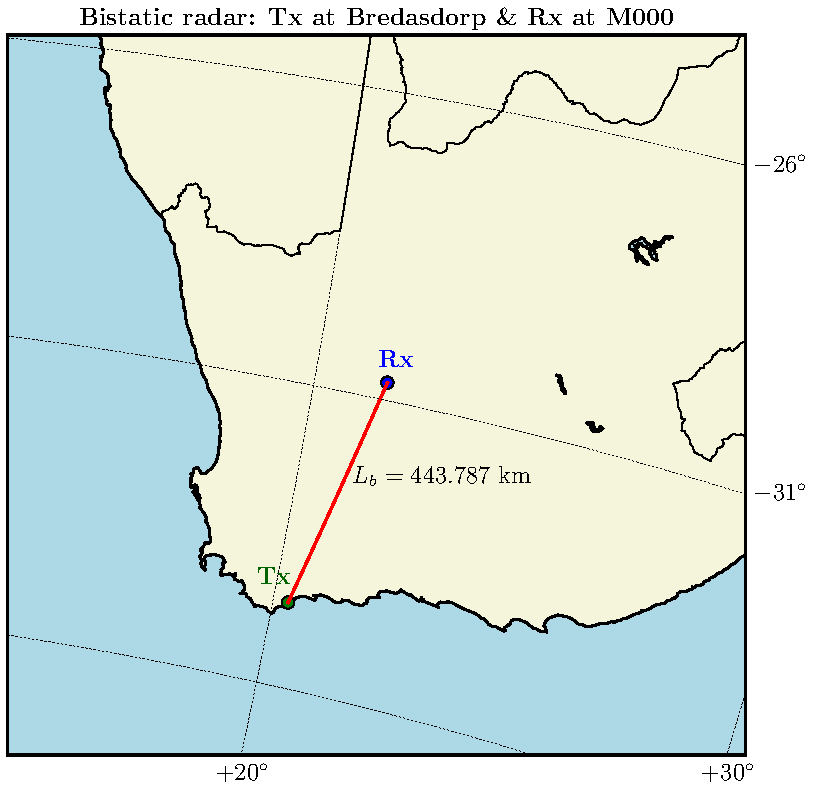
\includegraphics[scale=0.48]{bisradvisual.pdf}
	\caption{Map showing the location of the Tx in Bredasdorp at $34.6\mathrm{^\circ}\text{S}$ and $20.3\mathrm{^\circ}\text{E}$ and Rx at Carnarvon at $30.7\mathrm{^\circ}\text{S}$ and $21.4\mathrm{^\circ}\text{E}$.} 
	\label{fig:map}
\end{figure}
}

\frame[shrink]{\frametitle{The MeerKAT radio telescope}
\begin{figure}[t]
	\centering
	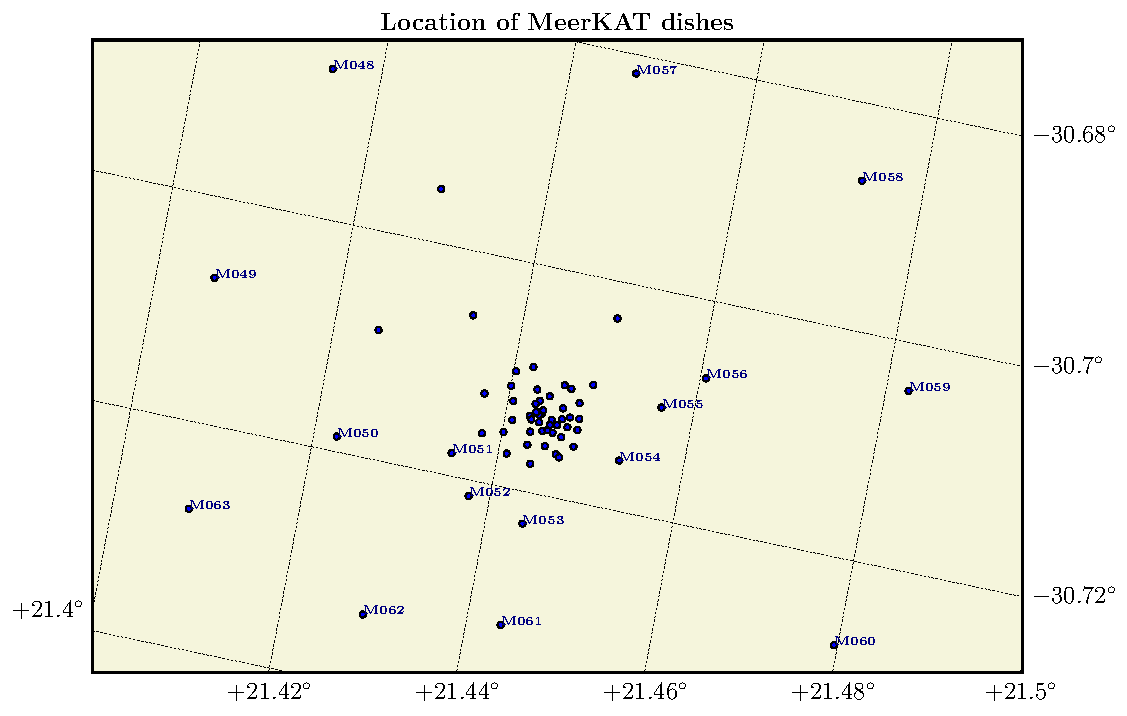
\includegraphics[scale=0.5]{meerkatlayout0.pdf}
	\caption{Map showing the layout of MeerKAT. The longest baseline is $7.697~\mathrm{km}$ (between \textbf{M048} 
	\& \textbf{M060} and between \textbf{M058} \& \textbf{M063}).} 
	\label{fig:meerkat}
\end{figure}
}

%\frame[shrink]{\frametitle{}}

%=====================================
\section[Bib]{Bibliography}
%\nocite{*}

\bibliographystyle{plainnat}
\bibliography{../bib/L12012}


%=====================================
\begin{frame}
\begin{center}
End lecture~\lecNo~\version.
\end{center}
\label{lastpg}
\end{frame}

\end{document}

%-------------------------------Lecture 9


